%========================================
% LESSON CONTENT: Conjuntos y Operaciones con Conjuntos
%========================================

\lesson{Conjuntos y Operaciones con Conjuntos}

\subsectiontitle{Introducción}

El ser humano tiende a crear colecciones. Hablamos de ``grupos de estrellas'' o ``constelaciones''. Nos atrae la idea de generalizar en ``grupos''.

En matemática esta tendencia a crear colecciones se representa utilizando el concepto de \textbf{conjunto}.

\begin{example}
\textbf{Ejemplos de Conjuntos en la Vida Cotidiana:}
\begin{itemize}
    \item \textbf{Música:} Conjuntos de notas musicales, conjuntos de músicos de salsa o rock
    \item \textbf{Arte:} Conjuntos de colores
    \item \textbf{Aritmética:} Al sumar dos números, se reúne un conjunto con otro
    \item \textbf{Estadística:} Al realizar una encuesta, se recopila un conjunto de datos
\end{itemize}
\end{example}

\subsectiontitle{Definiciones Básicas}

\begin{definition}
Un \textbf{conjunto} es una colección de objetos que tienen al menos una característica en común.

Nos referimos a los objetos que forman el conjunto como los \textbf{elementos del conjunto}.
\end{definition}

\begin{example}
Los \textbf{números naturales} son los números que usamos para contar:
$$\{1, 2, 3, 4, 5, \ldots\}$$

Este conjunto está bien definido. Sabemos sin ambigüedad cuáles son los elementos del mismo.
\end{example}

\subsectiontitle{Simbolismo y Notación}

\begin{itemize}
    \item \textbf{Letras Mayúsculas:} se usan para el nombre del conjunto
    \item \textbf{Letras minúsculas:} se usan para referirnos a elementos de un conjunto
\end{itemize}

\begin{example}
Llamemos $V$ al conjunto de las vocales:
$$V = \{a, e, i, o, u\}$$

\textit{Nota:} Enumeramos los elementos y usamos $\{ \}$ para incluir sus elementos.
\end{example}

\subsectiontitle{Formas de Representar Conjuntos}

\textbf{a) Enumeración (listas)}

Se enumeran los elementos del conjunto, separados por comas, y se incluyen entre llaves $\{ \}$.

\begin{example}
\begin{itemize}
    \item Números naturales: $\{1, 2, 3, 4, 5, \ldots\}$
    \item Números naturales pares: $\{2, 4, 6, 8, \ldots\}$
    \item Letras del alfabeto: $\{a, b, c, d, \ldots, x, y, z\}$
\end{itemize}
\end{example}

\textbf{b) Forma descriptiva}

Se describe mediante palabras y símbolos a los elementos del conjunto.

\begin{example}
\begin{itemize}
    \item Números naturales: $N = \{x \mid x \text{ es un número natural}\}$
    \item Números pares: $P = \{x \mid x \text{ es un número natural par}\}$
    \item Alfabeto: $A = \{x \mid x \text{ es una letra de nuestro alfabeto}\}$
\end{itemize}

\textit{Leemos:} ``A es el conjunto de todos los elementos x, tales que x es una letra de nuestro alfabeto''
\end{example}

\subsectiontitle{Pertenencia a un Conjunto}

\begin{definition}
\begin{itemize}
    \item Para indicar que un elemento \textbf{pertenece} a un conjunto: $\in$
    \item Para indicar que un elemento \textbf{no pertenece} a un conjunto: $\notin$
\end{itemize}
\end{definition}

\begin{example}
Usando los ejemplos anteriores:
\begin{align}
5 &\in N \\
5 &\notin P \\
p &\in A \\
7 &\notin A
\end{align}
\end{example}

\subsectiontitle{Relaciones entre Conjuntos}

\begin{definition}
\textbf{Conjuntos Equivalentes:} Si dos conjuntos $A$ y $B$ tienen la misma cantidad de elementos, son equivalentes:
$$A \sim B$$

\textbf{Conjuntos Iguales:} Si dos conjuntos $A$ y $B$ tienen exactamente los mismos elementos, son iguales:
$$A = B$$

\textbf{Conjunto Nulo:} Si un conjunto no tiene elementos:
$$\emptyset \quad \text{o} \quad \{ \}$$
\end{definition}

\begin{example}
\begin{itemize}
    \item $\{a, e, i, o, u\} \sim \{1, 2, 3, 4, 5\}$ (equivalentes)
    \item $\{a, e, i, o, u\} = \{u, o, a, e, i\}$ (iguales)
    \item $\{x \mid x \text{ es un número par mayor que 10 y menor que 12}\} = \emptyset$ (nulo)
\end{itemize}
\end{example}

\subsectiontitle{Subconjuntos}

\begin{definition}
Dados dos conjuntos $A$ y $B$, si todos los elementos del conjunto $A$ también pertenecen al conjunto $B$, se dice que $A$ es \textbf{subconjunto} de $B$:
$$A \subseteq B$$
\end{definition}

% Visual representation of subset relationship
\begin{center}
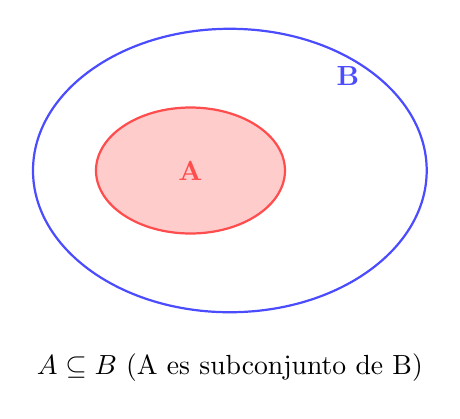
\begin{tikzpicture}[scale=1]
    % Set B (larger)
    \draw[thick, blue!70] (0,0) ellipse (2.5cm and 1.8cm);
    \node at (1.5,1.2) {\textcolor{blue!70}{\textbf{B}}};
    
    % Set A (smaller, inside B)
    \draw[thick, red!70, fill=red!20] (-0.5,0) ellipse (1.2cm and 0.8cm);
    \node at (-0.5,0) {\textcolor{red!70}{\textbf{A}}};
    
    \node at (0,-2.5) {$A \subseteq B$ (A es subconjunto de B)};
\end{tikzpicture}
\end{center}

\subsectiontitle{Operaciones con Conjuntos}

\begin{definition}
\textbf{Unión:} La unión de dos conjuntos $A$ y $B$, denotado $A \cup B$, es el conjunto de todos los elementos del conjunto $A$ y todos los elementos del conjunto $B$.

\textbf{Intersección:} La intersección de dos conjuntos $A$ y $B$, denotado $A \cap B$, es el conjunto de todos los elementos comunes entre el conjunto $A$ y el conjunto $B$.
\end{definition}

% Visual representation of union and intersection
\begin{center}
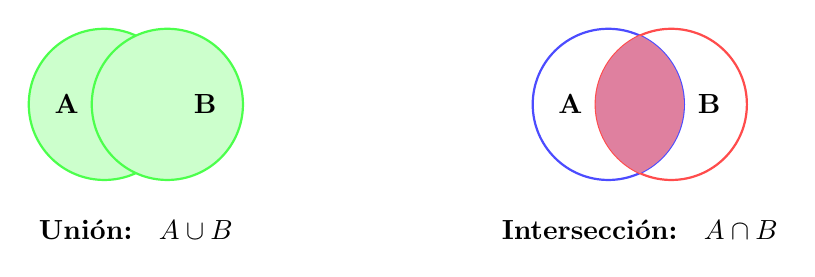
\begin{tikzpicture}[scale=0.8]
    % Union diagram
    \begin{scope}[xshift=-4cm]
        \draw[fill=green!20, draw=green!70, thick] (0,0) circle (1.2cm);
        \draw[fill=green!20, draw=green!70, thick] (1,0) circle (1.2cm);
        \node at (-0.6,0) {\textbf{A}};
        \node at (1.6,0) {\textbf{B}};
        \node at (0.5,-2) {\textbf{Unión: } $A \cup B$};
    \end{scope}
    
    % Intersection diagram
    \begin{scope}[xshift=4cm]
        \draw[draw=blue!70, thick] (0,0) circle (1.2cm);
        \draw[draw=red!70, thick] (1,0) circle (1.2cm);
        \begin{scope}
            \clip (0,0) circle (1.2cm);
            \fill[purple!50] (1,0) circle (1.2cm);
        \end{scope}
        \node at (-0.6,0) {\textbf{A}};
        \node at (1.6,0) {\textbf{B}};
        \node at (0.5,-2) {\textbf{Intersección: } $A \cap B$};
    \end{scope}
\end{tikzpicture}
\end{center}

\begin{example}
Considere los conjuntos: $A = \{-2, 7, 9\}$, $B = \{1, 9, 10, 30\}$, $C = \{-3, -2, -1\}$

\begin{align}
A \cup B &= \{-2, 1, 7, 9, 10, 30\} \\
A \cap B &= \{9\} \\
A \cap B \cap C &= \emptyset
\end{align}
\end{example}

\subsectiontitle{Conjuntos Numéricos}

\begin{definition}
\textbf{Números Naturales (Enteros Positivos):}
$$\mathbb{N} = \{1, 2, 3, 4, \ldots\}$$

\textbf{Números Enteros No Positivos:}
$$\{0, -1, -2, -3, \ldots\}$$

\textbf{Números Enteros:}
$$\mathbb{Z} = \{\ldots, -3, -2, -1, 0, 1, 2, 3, \ldots\}$$
\end{definition}

% Real numbers as union of rationals and irrationals
\begin{center}
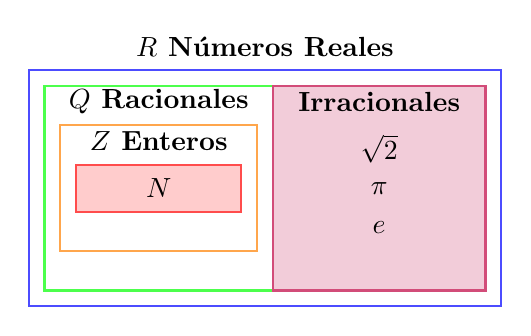
\begin{tikzpicture}[scale=1]
    % Outer rectangle for real numbers
    \draw[thick, blue!70] (-3,-1.5) rectangle (3,1.5);
    \node at (0,1.8) {\textbf{$\mathbb{R}$ Números Reales}};
    
    % Left side: Rationals with nested structure
    \draw[thick, green!70] (-2.8,-1.3) rectangle (0.1,1.3);
    \node at (-1.35,1.1) {\textbf{$\mathbb{Q}$ Racionales}};
    
    % Integers inside rationals
    \draw[thick, orange!70] (-2.6,-0.8) rectangle (-0.1,0.8);
    \node at (-1.35,0.6) {\textbf{$\mathbb{Z}$ Enteros}};
    
    % Naturals inside integers
    \draw[thick, red!70, fill=red!20] (-2.4,-0.3) rectangle (-0.3,0.3);
    \node at (-1.35,0) {\textbf{$\mathbb{N}$}};
    
    % Right side: Irrationals
    \draw[thick, purple!70, fill=purple!20] (0.1,-1.3) rectangle (2.8,1.3);
    \node at (1.45,1.1) {\textbf{Irracionales}};
    \node at (1.45,0.5) {$\sqrt{2}$};
    \node at (1.45,0) {$\pi$};
    \node at (1.45,-0.5) {$e$};
\end{tikzpicture}
\end{center}

La relación de inclusión es:
$$\mathbb{N} \subset \mathbb{Z} \subset \mathbb{Q} \subset \mathbb{R}$$

\subsectiontitle{Números Primos y Compuestos}

\begin{definition}
\textbf{Factor o Divisor:} Un número $m$ es factor o divisor de un número natural $n$ si:
\begin{itemize}
    \item $m \times r = n$ (para algún entero $r$)
    \item $n$ dividido por $m$ da un entero, con residuo cero
\end{itemize}

\textbf{Número Primo:} Un número natural diferente de 1 cuyos únicos factores son 1 y el número mismo.

\textbf{Número Compuesto:} Un número natural mayor de 1 que no es primo.
\end{definition}

\begin{example}
\begin{itemize}
    \item 3 es factor de 15, pues $3 \times 5 = 15$
    \item Los primeros números primos: $2, 3, 5, 7, 11, 13, \ldots$
    \item Los primeros números compuestos: $4, 6, 8, 9, 10, 12, \ldots$
    \item Factorización prima de 12: $12 = 2 \cdot 2 \cdot 3 = 2^2 \cdot 3$
\end{itemize}
\end{example}

\subsectiontitle{Números Racionales e Irracionales}

\begin{definition}
\textbf{Número Racional:} Un número que puede escribirse de la forma $\frac{a}{b}$, donde $a, b$ son enteros y $b \neq 0$.

\textbf{Número Irracional:} Un número que no se puede expresar como una fracción. Su representación decimal no es finita ni periódica.
\end{definition}

\begin{example}
\textbf{Números Racionales:}
\begin{itemize}
    \item $\frac{3}{4}$, $6 = \frac{6}{1}$, $12.5 = \frac{125}{10}$
    \item Decimales periódicos: $0.333\ldots = \frac{1}{3}$, $2.333\ldots = \frac{7}{3}$
\end{itemize}

\textbf{Números Irracionales:}
\begin{itemize}
    \item $\sqrt{2} \approx 1.41421356\ldots$
    \item $\pi \approx 3.14159265\ldots$
    \item $e \approx 2.71828182\ldots$
\end{itemize}
\end{example}